\documentclass[logo,reportComp]{thesis}
\usepackage[cpp,pseudo]{mypackage}

\title{高级编程技术实验报告}
\subtitle{实验四:密码}
\school{数据科学与计算机学院}
\author{陈鸿峥}
\classname{17大数据与人工智能}
\stunum{17341015}
\headercontext{高级编程技术实验报告}
% \authorremark{本实验报告用\LaTeX撰写,创建时间:\builddate\today}

\begin{document}

\maketitle

\section{问题描述及求解思路}
利用面向对象编程(OOP)实现简单的编码解码器。

\subsection{字符串重排}
利用递归给出一个字符串的所有重排列(permutation)。

实施方法:
\begin{itemize}
	\item 基情况:当字符串长为1时,即单个字符,返回它自己。
	\item 递归情况:将字符串首个字符(head)取出,依次插入后续的字符串(tail),进而得到新的字符串。注意插入字符的过程采用Python的\textbf{列表解析}完成。
\end{itemize}

\subsection{Caesar编码}
实现基类\verb'Message',以及两个子类\verb'PlaintextMessage'、\verb'CiphertextMessage'。

基类方法:
\begin{itemize}
	\item \verb'__init__':初始化函数,直接将输入参数赋值给成员函数即可
	\item \verb'get_message_text'、\verb'get_valid_words':均直接返回成员函数。注意由于Python共享对象的机制,后者需要返回一个copy,防止原来的值被修改
	\item \verb'build_shift_dict':创建一个偏移后的字母对应/字典。利用Python内置字符串函数\verb'find'可以找出每一个字母在原字符串\verb'string.ascii_lowercase'的位置,进而通过
	\begin{center}\verb'new_char = (alpha.find(c)+shift) % 26'\end{center}
	可得到新的字母
	\item \verb'apply_shift':利用上面创建的映射表,将原来的字母更改为新的字母。注意考虑空格等非字母的情况,故需要用\verb'alphabet.get(c,0)'来防止出错
\end{itemize}

子类方法:
\begin{itemize}
	\item \verb'__init__':先调用父类方法\verb'Message.__init__(self,text)'进行初始化,然后再初始化子类成员
	\item \verb'get'方法:直接返回成员,同样注意\verb'dict'要返回拷贝
	\item \verb'decrypt_message':枚举所有0到25的偏移量,并将该偏移量应用到字符串中,计数偏移出来的字符串有多少合法单词(用\verb'split'进行字符串分割),记录下最多合法单词的偏移量及字符串,该值即为所求。注意如果原来的偏移量是$s$,那么最优的偏移量即为$26-s$。
\end{itemize}

\subsection{替代编码}
采用替代码进行编码和解码,实施父类\verb'SubMessage'和子类\verb'EncryptedSubMessage'。

这里只阐述与Part B不同的部分,父类:
\begin{itemize}
	\item \verb'build_transpose_dict':构造一个字典\verb'res',并枚举每一个字母,如果是元音,则进行映射,否则保持原字母。
	\item \verb'apply_transpose':与Part B相同
\end{itemize}

子类:
\begin{itemize}
	\item \verb'decrypt_message':利用Part A的字符串排列函数\verb'get_permutation'将\verb'VOWELS_LOWER'和\verb'VOWELS_UPPER'都进行重排作为\verb'perm',并将每一个\verb'perm'传入\verb'build_transpose_dict'并应用。通过计数解码的字符串有多少合法单词(用\verb'split'进行字符串分割),记录下最多合法单词的字符串并返回。
\end{itemize}

\section{代码}
代码实施及注释请见附件\verb'ps4a.py'、\verb'ps4b.py'、\verb'ps4c.py'。

\section{运行截图}
实验运行结果如下面几幅图片所示,\textbf{注意给出了多个自己写的复杂测试样例,确保结果的正确性和鲁棒性}。
\begin{figure}[H]
\centering
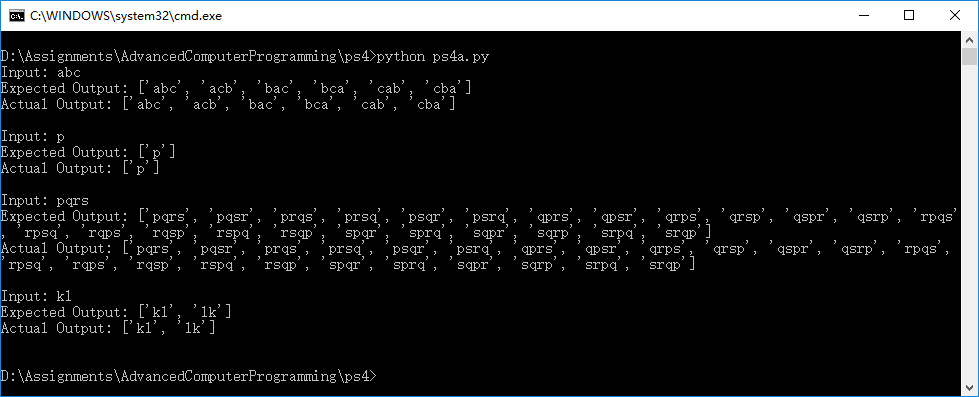
\includegraphics[width=\linewidth]{fig/permutation.PNG}
\caption{Part A结果,给出测试样例和多个自己写的样例输出}
\end{figure}
\begin{figure}[H]
\centering
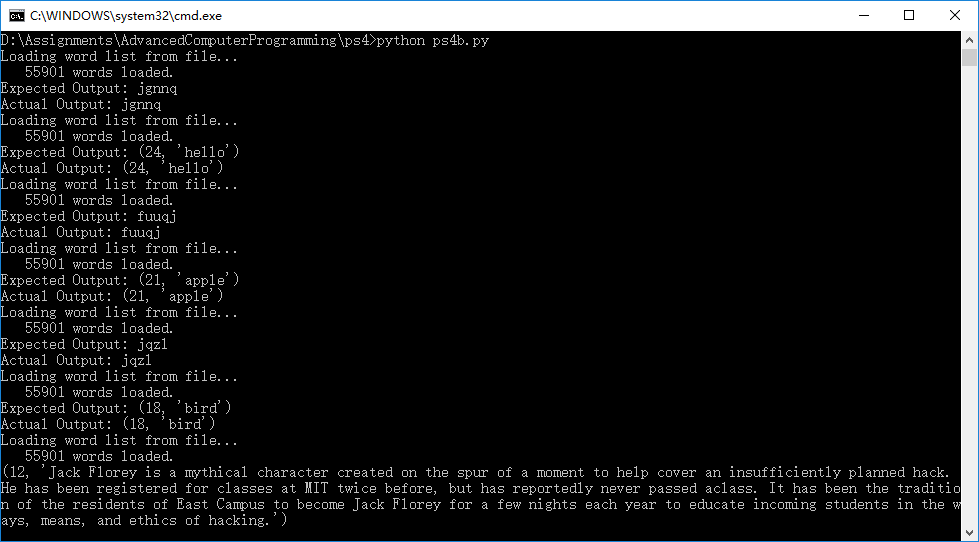
\includegraphics[width=\linewidth]{fig/partb.PNG}
\caption{Part B结果,给出测试样例和多个自己写的样例输出}
\end{figure}
\begin{figure}[H]
\centering
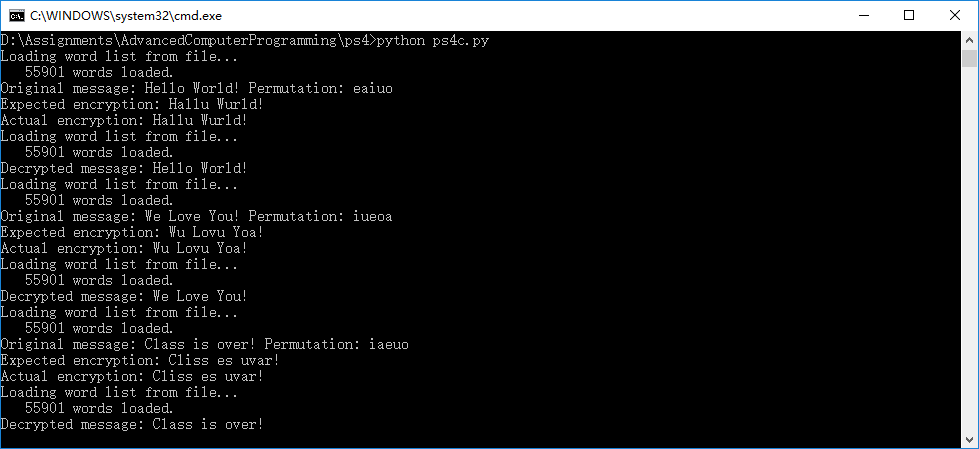
\includegraphics[width=\linewidth]{fig/partc.PNG}
\caption{Part C结果,给出测试样例和多个自己写的样例输出}
\end{figure}

\end{document}

% 实验提交内容
% 邮件主题,作业文件命名规范(学号、姓名)
% 文档pdf格式(问题、求解思路、代码、注释、运行截图)
% 考虑健壮性、可读性
% 极端样例